\section{Background}

\subsection{Edge Computing}
\glsresetall%

\begin{figure}
    \centering
    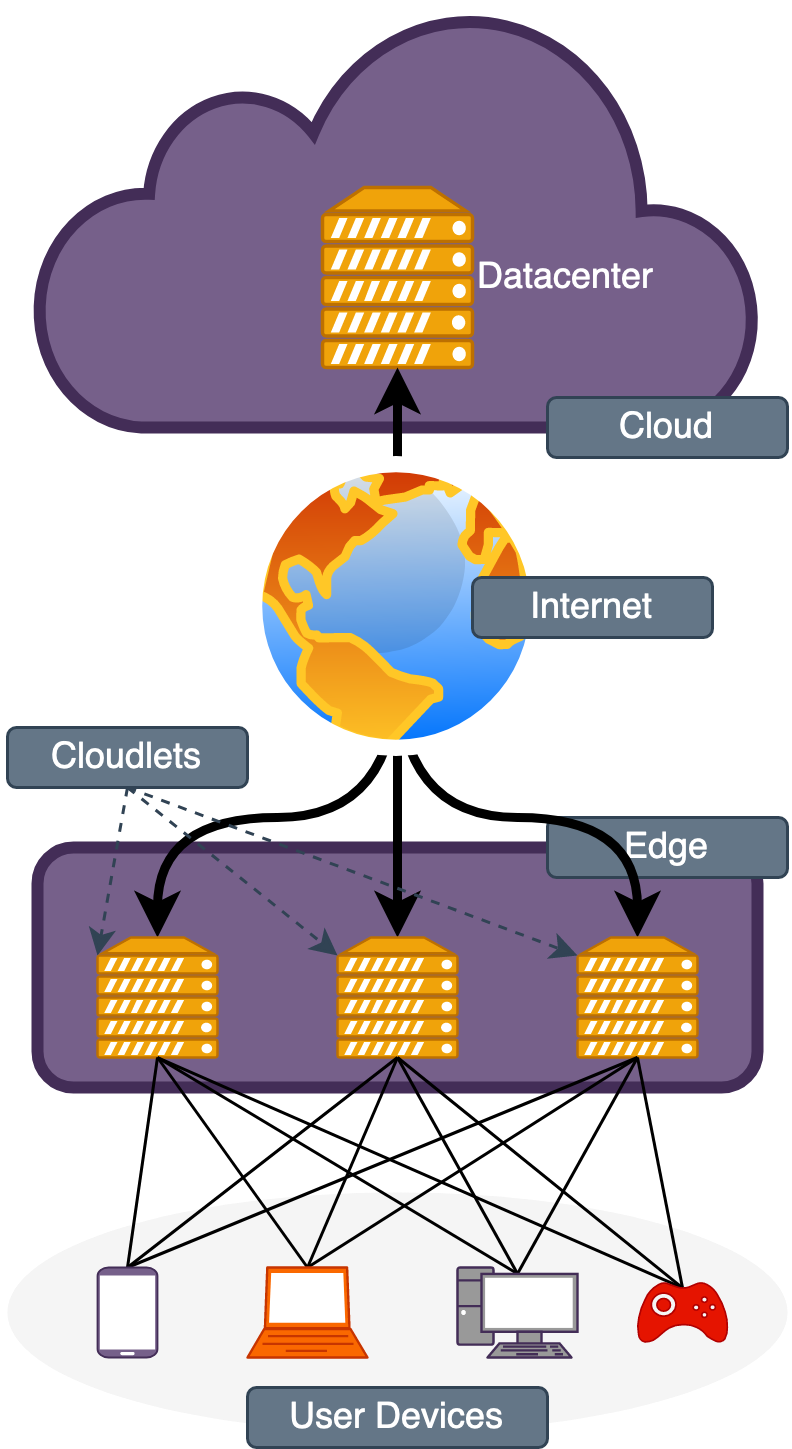
\includegraphics[height=30em]{figures/edgecomputing}
    \caption{%
        Conceptual design of Edge Computing.
        Compute nodes are placed a at the edge of the network, a few hops away from end users.
        In other words, compute is located between users and the internet and the Cloud.
    }\label{fig:edgecomputing}
\end{figure}


Edge Computing is a novel distributed computing paradigm, emerging from a need to overcome the drawbacks of offloading computation and data to the Cloud.
Cloud computing, the reigning distributed computing model, allows users to access shared pools of resources such as servers, databases, and applications, over the internet~\cite{gai2012towards}.
These pools of resources are managed in a centralized manner by specialized providers, and users and businesses can access them on-demand, without having to invest in and manage infrastructure of their own.
Providers in turn employ economies of scale, providing these services by deploying massive amounts of computing power and storage capacity in specialized locations known as datacenters.
These hardware resources are then further compartmentalized through the use of virtualization technologies such as \glspl{VM} and containers~\cite{gai2012towards}.

Through this design, Cloud computing affords significant advantages to users.
As services are deployed in a centralized manner accessible over the internet, users can interact with their data and applications from anywhere in the world, from any device.
Thanks to economies of scale and virtualization technologies, the Cloud is highly scalable;
services can be scaled simply by spawning more \glspl{VM}.
The specialized nature of Cloud providers, the scale of modern datacenters, and the use of virtualization also make the Cloud highly reliable.
When hardware fails, recovering is simply a matter of migrating the service container or \gls{VM} to an available compute node~\cite{endo2016high}.

However, the Cloud is not suitable for everything, and presents important drawbacks and challenges for latency-sensitive and/or bandwidth-intensive applications.
In order to achieve the necessary economies of scale, Cloud datacenters are designed to serve users distributed across vast geographical areas.
These installations are thus often located ``far'' from potential users;
for instance, at the time of writing, \gls{AWS} processes traffic from all of Scandinavia and the Baltic countries through a single datacenter in Stockholm~\cite{awsregions}.
This leads to prohibitively high latencies for both highly interactive immersive applications such as mobile \gls{XR} and for \glspl{CPS} and \glspl{NCS}~\cite{tolia2006quantifying,lagar2007interactive,satyanarayanan2009case,varghese2016challenges,shi2016promise}.
The former category requires \emph{motion-to-photon} latencies (i.e.\ time between input capture and feedback) below \SI{60}{\milli\second} for interactions to be perceived as fluid and responsive by the user~\cite{chen2017empirical}; the latter can require sub-\SI{10}{\milli\second} latencies, for instance in the case of vehicular safety systems.
Such latencies are unfeasible to consistently achieve with Cloud computing~\cite{dang2021cloudy}.
On the other hand, as smart devices, appliances, and sensors become more and more ubiquitous, the network architectures of modern datacenters face increasing challenges to deal with the massively increasing volume of traffic~\cite{shi2016edge,wang2019towards}.

\medskip
Edge Computing emerges as a potential answer to these challenges~\cite{satyanarayanan2009case,shi2016promise,shi2016edge,varghese2016challenges,satyanarayanan2017emergence,bittmann2017edge,wang2019towards}.
The foundation for this concept was laid by \citeauthor{satyanarayanan2009case}~\cite{satyanarayanan2009case} in\ \citeyear{satyanarayanan2009case}.
To tackle the prohibitively high latencies of Cloud computing, the authors proposed an extension of the existing Cloud computing paradigm with compute nodes at the edge of the Internet.
Instead of offloading computation to a datacenter potentially thousands of kilometers away, in Edge Computing it is offloaded to a compute node at the \emph{edge} of the network close to the user, see \cref{fig:edgecomputing}.

The architecture of Edge Computing offers several advantages, the primary being the significant reduction of latency.
Edge Computing can serve highly latency-sensitive and resource-intensive applications with extremely low latencies while still providing orders of magnitude more computing and energy resources than those present on mobile and wearable devices.
Another important advantage of this design is bandwidth reduction.
Edge application traffic either does not need to traverse the public internet, or it can be aggregated and compressed at the Edge before uplink transmission.

% Please add the following required packages to your document preamble:
% \usepackage{booktabs}
% \usepackage{graphicx}
\begin{table}[]
    \centering
    \caption{Comparison between Cloud Computing and three implementations of Edge Computing.}\label{tab:cloud-vs-edge}
    \tiny
    \renewcommand{\arraystretch}{1.5}
    \begin{tabularx}{\textwidth}{@{}lYYYY@{}}
        \toprule
        &
        \textbf{Cloud} &
        \textbf{Cloudlet} &
        \textbf{\acs{MEC}} &
        \textbf{Fog} \\ \midrule
        \textbf{Location} &
        Data centers that are geographically distant from end-users. &
        Micro-datacenters close to end-users. &
        Integrated within the \acs{RAN}. &
        Distributed across the Edge-Cloud network continuum. \\
        \textbf{Latency} &
        \ensuremath{> \SI{50}{\milli\second}} &
        \ensuremath{\leq \SI{50}{\milli\second}} &
        \ensuremath{\leq \SI{10}{\milli\second}} &
        \ensuremath{\leq \SI{50}{\milli\second}} \\
        \textbf{Resources} &
        Limited only by network bandwidth and latency. &
        \multicolumn{3}{%
            >{\hsize=\dimexpr3\hsize+4\tabcolsep+2\arrayrulewidth\relax}Y%
        }{Limited, but orders of magnitude more than end-user devices.} \\
        \textbf{Security} &
        Relies on strong network and perimeter defenses. &
        \multicolumn{3}{%
            >{\hsize=\dimexpr3\hsize+4\tabcolsep+2\arrayrulewidth\relax}Y%
        }{Data can be kept close to the source and encrypted.} \\
        \textbf{Privacy} &
        Data is aggregated and stored centrally. &
        \multicolumn{3}{%
            >{\hsize=\dimexpr3\hsize+4\tabcolsep+2\arrayrulewidth\relax}Y%
        }{Data can be kept locally, reducing the risk of exposure.} \\
        \textbf{Scalability} &
        Easily scalable by adding more resources to datacenters. &
        \multicolumn{3}{%
            >{\hsize=\dimexpr3\hsize+4\tabcolsep+2\arrayrulewidth\relax}Y%
        }{Limited by virtue of Edge nodes being distributed and energy-constrained in comparison to datacenters.} \\
        \textbf{Use~Cases} &
        Large-scale systems that are not latency-sensitive or do not require real-time processing. &
        Latency-sensitive applications such as \acs{CPS} and \acs{AR}. &
        Latency-sensitive applications in mobile and wearable contexts. &
        \acs{IOT} \\ \bottomrule
    \end{tabularx}%
\end{table}

\Cref{tab:cloud-vs-edge} shows an overview of the differences between Cloud Computing and three implementations of Edge Computing, \emph{Cloudlet}-based Computing, \gls{MEC}, and \emph{Fog} Computing.
The first of these corresponds to the original Edge Computing concept as introduced in~\citeauthor{satyanarayanan2009case}.
It is based on the idea that Edge compute capabilities will be realized through geographically distributed micro-datacenters known as \emph{cloudlets}.
Cloudlets have been envisioned as featuring most of the key characteristics of Cloud datacenters, such as multi-tenancy, virtualization of computing resources, virtually unrestricted access to energy, as well as limited scalability, all while being one or two hops away from the user.
This design builds on previous work on \emph{cyber foraging}~\cite{noble1997agile,flinn1999energy,satyanarayanan2001pervasive}.
Cyber foraging refers to the extension and amplification of the capabilities of mobile and wearable devices by offloading computation and data manipulation to nearby infrastructure (as opposed to distant infrastructure such as the Cloud).

\glsreset{MEC}%
\glsreset{RAN}%
In later years, an extension to Edge Computing denoted \gls{MEC} has emerged, which pairs Edge Computing with novel mobile networking standards such as 5G~\cite{hassan2019edge,pham2020survey,wan2020efficient}.
A modern mobile network is composed of two main components: the \gls{RAN} and the core network.
The former includes the base stations and other wireless communication equipment to which user's equipment (i.e.\ mobile phones, mobile internet dongles, etc.) connect. 
The \gls{RAN} provides access to the core network, which in turn routes data between \glspl{RAN}, handles billing and authentication, and provides access to external services such as the internet and the Cloud.
\gls{MEC} is defined as an Edge Computing deployment in which Cloud-like compute is deployed within the \gls{RAN} of a mobile network.
Compute power is never more than a single wireless hop away from users application traffic thus never enters the core or the public internet.
This architectural design has the potential to enable unprecedented use-cases requiring stringent, sub-\SI{10}{\milli\second} latency bounds and high bandwidths.
Two examples of such applications, of relevance for the present work, are \acl{WCA}~\cite{ha2014towards,chen2018application,wang2020scaling,chen2017empirical,chen2018application} and \aclp{NCS}~\cite{sasaki2016vehicle,wang2018bandwidth,wan2020efficient}.
These applications had been hitherto inviable to implement due to the limitations of Cloud offloading in mobile and wearable contexts, but have now become a practical reality thanks to \gls{MEC}.

Finally, another variant of Edge Computing called \emph{Fog} computing, introduced by \citeauthor{bonomi2012fog}~\cite{bonomi2012fog} in\ \citeyear{bonomi2012fog}, concerns itself specifically with the distribution of computing power between the Cloud and the edge for the reduction of bandwidth requirements.
By aggregating, transforming, and filtering data at multiple levels in the network, Fog computing aims to reduce the load placed on Cloud datacenters by massive \gls{IOT} sensor networks~\cite{yi2015survey}.
Edge Computing also presents opportunities for increased data security, privacy, and integrity, by keeping it geographically close to its origin and by allowing for anonymization through denaturing and local aggregation before offloading to Cloud services~\cite{satyanarayanan2017emergence}.

\subsection{Performance evaluation of networked systems}

Performance evaluation is an essential step in designing and optimizing networked systems, in order to ensure efficient and effective operation.
Such evaluation involves measuring and analyzing system performance under a multitude of scenarios to identify potential bottlenecks.
In practice, three main approaches exist to the performance evaluation of any complex system; analytical modeling, simulations, and experimental evaluation~\cite{fernandes2017performance}.
These approaches each have their advantages and disadvantages.

Analytical or mathematical modeling involves creating a mathematical model that represents the system's behavior and performance.
This involves defining the system's components, their interactions, and the performance metrics used to measure the system's performance.
The mathematical model can be solved analytically, providing insights into the behavior of the system under different conditions.

Analytical modeling is often used as a first step when attempting to identify possible solutions to a problem and provide an initial reduction of the problem space.
One of the key advantages of mathematical modeling is that their realism and resulting complexity can be arbitrarily constrained as required.
This allows researchers to quickly evaluate a large number of scenarios by employing coarse, approximate models to identify and highlight latent issues.
These models can then be refined to further narrow the solution space.
This approach is particularly useful for systems with complex interactions between multiple components, where testing every possible scenario in the real world or even in simulations would be impractical or impossible due to time and cost constraints.

However, analytical modeling also has its limitations, in particular with respect to highly complex systems.
In systems involving a large number of interacting components and processes, the mathematical equations required to model the system become more complex and difficult to solve.
Assumptions about system behavior also become more inaccurate and incomplete as this behavior grows in complexity.
As mathematical models are based on assumptions about the system's behavior and performance, incorrect, incomplete, or inaccurate assumptions can in turn lead to erroneous predictions.
Additionally, complex systems may involve non-linear interactions between components, further increasing the difficulty of accurately modeling these systems.

\medskip

The second possible approach to performance evaluation of networked systems is simulation.
This involves creating a computational model of the system, and then using it to simulate a series of scenarios to measure the model's performance.
Simulations are often used to validate mathematical models and further narrow down the problem and solution spaces.

Simulations offer numerous advantages.
They represent an inexpensive and reliable way to study systems, by providing safe, controlled, and repeatable environments in which to test the system's behavior~\cite{fernandes2017performance}.
Simulations also allow researchers to evaluate the system's performance with a high degree of accuracy and granularity, as they can approximate the system's behavior at a very fine-grained level without necessarily having to resort to complex mathematical modeling.
Additionally, simulations can be used to test the impact of changes to the system's design or configuration, allowing researchers and system designers to identify the most effective solutions to improve performance.

Simulation is a widely used and well-established method in networked system research, and there exists a rich literature surrounding tools for its implementation as a methodology~\cite{wehrle2010modeling}.
The availability of simulation frameworks has made it easier for researchers to evaluate the performance of networked systems controlled environments.
These frameworks provide a set of tools and libraries that enable researchers to create models of networked systems with very little overhead to simulate their behavior.

Examples of frameworks for network simulation include the widely adopted \acs{OMNET}~\cite{omnet}, \acs{ns2}, and \acs{ns3}~\cite{nsnam} discrete-event simulators.
\acs{OMNET} is an open-source, modular, and extensible discrete-event simulator that provides an object-oriented framework for modeling and simulating networks, and includes a variety of modules for different network protocols and technologies.
\acs{ns2}, and \acs{ns3} refer to two generations of the same project.
These widely popular simulation frameworks provide comprehensive sets of tools for modeling and simulating networks, and include support for a range of network technologies.

Nevertheless, simulations also have their limitations.
The realism of simulations is inherently limited by the accuracy and completeness of the underlying models used.
Simulations rely on mathematical models that are an abstraction of the real-world system, and these models are only as accurate as the assumptions made and the data used to construct them.
Simulations also cannot account for the impact of external factors on the system's performance.
Real-world systems are often subject to factors that cannot be modeled accurately, such as unpredictable weather conditions, human behavior, or hardware failures.
Moreover, for complex systems with many interacting components, simulations can become prohibitively computationally expensive and time consuming.
It is not unusual for simulations of highly complex systems to execute much slower than real-time due to the computational power required to calculate the interactions between elements in the system.

\medskip

The third and final approach to performance evaluation of networked systems is practical experimentation on the real system.
Such an approach involves measuring the performance of the \emph{real} system using practical, real-world experiments in different scenarios.
Experimental research is often the final stage in systematic performance benchmarking, employed once the problem space has been reduced to a handful of potential solutions through mathematical modeling and subsequent simulations.

Experimental research provides the most accurate assessment of system performance.
It allows for an extremely high level of realism and can capture factors that cannot be accurately modeled through mathematical modeling or simulations, such as non-linear behaviors, human behavior, and unexpected events.
Experimental methods provide direct measures of the system's performance under real-world conditions, enabling researchers to validate the accuracy of their mathematical models and simulations.

However, experimental approaches also come with challenges, such as cost, practicality, repeatability, and replicability.
Experimental research is often time-consuming and expensive to perform, as its implementation requires access to the real system under study.
Additionally, experimental research is also limited in terms of replicability and repeatability, particularly for systems subject to external factors or stochastic and chaotic effects.
This can make it challenging to draw definitive conclusions from experimental research.

When it comes to experimental approaches in research involving humans, there are additional challenges that must be considered beyond those mentioned above.
Ethical concerns related to participant safety, informed consent, and privacy must be addressed, and studies involving human participants must be reviewed and approved by appropriate ethical review panels\footnote{%
    In Sweden, ethical review is handled at the state level by the Ethical Review Authority (\emph{Etikprövningsmyndigheten}); in the \acs{USA}, it is handled by each institution's \gls{IRB}.
}.
Recruitment and retention of human participants can be challenging, as participants may drop out or not show up for study sessions, leading to data collection difficulties.
Despite these challenges, research involving human participants provides invaluable insights into the behavior and performance of networked systems and is critical for fully understanding and optimizing the performance of these systems in real-world settings.

\subsection{Closed-loop feedback systems enabled by Edge Computing}

\todo[inline]{Write an intro?}

\subsubsection{\glsfmtlong{XR}}\label{background:xr}
\todo[inline]{Needs citations.}
\glsreset{XR}
\glsreset{AR}
\glsreset{VR}
\glsreset{MR}

\gls{XR} is an umbrella term used to refer to all immersive technologies that combine real and virtual environments, including technologies such as \gls{AR}, \gls{VR}, and \gls{MR}.
\emph{Immersiveness} refers to the extent to which a technology can fully engage a user's senses to create the illusion of being in a different environment or situation.
A highly immersive experience can make the user feel like they are physically present in a different world or reality.

\gls{AR} merges digital content with the physical world, enhancing human perception and cognition through the overlay of virtual objects and information on top of the real environment.
This technology can superimpose tooltips, virtual \gls{2D} and \gls{3D} objects, or even full-fledged videos on top of what the user sees.
These overlays are most often presented to the user through wearable or mobile devices, such as smartphones or smart glasses (e.g. Google Glass).
To create an \gls{AR} experience, the device's camera captures the real-world environment, and the image feed is processed in real-time in software.
The digital objects are then superimposed onto the real-world view and displayed on the device's screen, where they can optionally be interacted with by touching the screen or using voice commands.
Other sensors can also be used to track the user's movements and position, and adjust the digital objects accordingly.

\gls{VR}, on the other hand, takes it a step further and involves forgoing the real world, completely immersing the user in a fully virtual environment.
Due to its deeply immersive nature, \gls{VR} requires users to wear specialized equipment such as a \gls{VR} headset.
The headset contains two high-resolution displays (one for each eye) and a set of headphones, and is connected to a computer or a gaming console, which generates the virtual environment in real-time.
The headset tracks the user's head movements and adjusts the virtual displays accordingly to create the illusion of being in a completely immersed in a different world.
Objects in the virtual environment can be interacted with either through the use of special hardware such as instrumented gloves or controllers, or by using sensors which track the user's hands.
Some advanced \gls{VR} platforms even include omnidirectional treadmills which allow the users navigate the virtual world by walking, running, and even jumping. 

Finally, \gls{MR} combines elements from both aforementioned technologies.
Like \gls{VR}, \gls{MR} uses a headset with high-resolution displays and sensors to track the user's movements.
However, \gls{MR} headsets also contain cameras that capture the real-world environment, in order to overlay digital objects onto the real world as in \gls{AR}.
These objects are rendered in real-time and projected onto the real-world view in the user's headset in a seamless and realistic way.
In this way, \gls{MR} creates a hybrid environment where users can interact with both virtual and real-world elements simultaneously, resulting in an illusion of natural interaction between users and digital elements.

% Please add the following required packages to your document preamble:
% \usepackage{booktabs}
\begin{table}[]
    \centering
    \caption{Comparison between different \acs{XR} technologies.}
    \label{tab:xrcomparison}
    \tiny
    \renewcommand{\arraystretch}{1.5}
    \begin{tabularx}{\textwidth}{@{}lYYY@{}}
        \toprule
        &
        \textbf{\acl{VR}} &
        \textbf{\acl{AR}} &
        \textbf{\acl{MR}} \\ \midrule
        % \textbf{Definition} &
        % A technology that creates a completely digital environment that simulates a real-world experience &
        % A technology that superimposes digital objects on the real world &
        % A technology that combines digital objects with the real world in a seamless way \\
        \textbf{Immersiveness} &
        High &
        Medium &
        Medium to high \\
        \textbf{User Interaction} &
        Only with the digital world &
        Both with the real and digital worlds &
        Both with the real and digital worlds in a seamless way \\
        \textbf{Equipment Required} &
        Headset and controllers &
        Smartphones, tablets, or \acs{AR} glasses &
        Headset and controllers \\
        % \textbf{Use Cases} &
        % Gaming, education, and training &
        % Retail, entertainment, education, and gaming &
        % Industrial design, engineering, and military training \\
        \textbf{Advantages} &
        Provides realistic immersive experience in a completely digital environment that can be easily adapted and changed. &
        Can be implemented cheaply on massively-available technology such as smartphones. &
        Provides a combination of AR and VR benefits, allowing seamless interaction between real and virtual worlds. \\
        \textbf{Drawbacks} &
        Isolates users from the real world, may cause motion sickness, and requires expensive equipment. &
        Limited field of view, reliance on external environment, and not fully immersive. &
        Expensive, complex, and may cause visual discomfort \\
        \textbf{\acs{QoS} Requirements} &
        High bandwidth, low latencies.
        Delay and jitter can lead to motion sickness. &
        Low latencies to ensure accurate, real-time overlay of digital assets. &
        High bandwidth, low latencies.
        Delay and jitter can lead to motion sickness. \\
        \bottomrule
    \end{tabularx}
\end{table}

A comparison of select characteristics of \gls{VR}, \gls{AR}, and \gls{MR} is presented in \cref{tab:xrcomparison}.
A key factor in which these applications differ is in their respective \gls{QoS} requirements.
Out of the three, \gls{AR} has the least stringent requirements.
\gls{AR} in particular does not require a high bandwidth, as only individual digital objects are generated.
However, low latencies are still a requirement, in order to ensure that the superimposition of the digital objects on top of the real-word view is accurate and in real-time.
In addition, \gls{AR} requires a high level of accuracy in tracking the user's movements and the position of the device's camera, as inaccuracies can lead to misalignment between the real-world view and the digital objects, leading to degraded \gls{QoE}.

\gls{VR}, on the other hand, requires a high level of \gls{QoS} in terms of both latency and bandwidth to deliver a smooth, highly immersive, and realistic experience.
Moreover, delays or jitter in \gls{VR} experiences can lead to motion sickness in users.
The user's movements and interactions must thus be tracked and rendered accurately in real-time, which requires low latencies between the headset and the computing device.
A high bandwidth is also necessary to transmit high-resolution graphics and audio back to the headset.
Given the similarities between the technologies, these same requirements also apply to \gls{MR}.

\medskip

Due to their ability to create immersive experiences for users and closely mimic and simulate real-life scenarios, \gls{XR} systems have found applications across a wide spectrum of industries and fields.
One of the most common uses of these technologies can be found in the domain of entertainment.
\gls{VR} allows users to become fully immersed in virtual experiences, including games, concerts, movies, making them feel almost physically present without having to leave the comfort of their homes.
Further, \gls{AR} and \gls{MR} allow for the merging of the virtual and real worlds, bringing entertainment to life in users day-to-day surroundings.
The popularity of this approach can be clearly seen in the explosive success of modern mobile \gls{AR} games such \citetitle{pokemongo}~\cite{pokemongo}.

\gls{XR} also presents tremendous opportunities for education and training.
Through the use of these technologies, students can get hands-on yet safe, simulated experience in a multitude of scenarios.
\gls{VR} is leveraged, for instance, in the training of new medical professionals, allowing students to learn anatomy and practice surgical procedures in realistic virtual environments.
On the other hand, \gls{AR} and \gls{MR} are employed in manufacturing, to train and assist technicians in highly specialized assembly lines.
Workers can receive real-time guidance through \gls{AR}-enabled headsets, improving accuracy and safety while controlling machine operations on the factory floor.
\gls{AR} can also provide augmented, step-by-step guidance for maintenance and repair of equipment, augmenting thus the capabilities of workers and the productivity of the workplace as a whole.

\paragraph{\glsfmtlong{WCA}}\label{sec:background:wca}
\glsreset{WCA}

Of particular interest for this dissertation is a particular subset of \gls{AR} denoted \acf{WCA}, a technology designed to provide real-time support and guidance to individuals performing complex tasks in a plethora of domains.
Designed to be deployed on wearable devices, \gls{WCA} overlays digital information onto the real world and provides context-aware feedback to users, in order to assist and guide them in to efficiently complete a task~\cite{ha2014towards,chen2015early,chen2018application,wang2020scaling}.

Originally motivated by assistive use-cases for individuals with reduced cognition due to illness, injury, or age, \gls{WCA} technology has evolved to include the enhancement of the cognitive abilities of users in areas such as manufacturing, healthcare, and aviation.
Among the primary benefits of this technology is that it can help reduce the cognitive load on individuals performing complex tasks.
By providing real-time guidance and support, it can improve accuracy and speed of task completion, reduce errors and minimize the risk of accidents.
For example, a \gls{WCA} could help a technician performing maintenance on an aircraft by displaying relevant technical information about the aircraft parts and step-by-step instructions on how to perform complex specific repairs.
\gls{WCA} is a promising technology that has the potential to revolutionize the way we perform complex tasks.
As the technology continues to evolve and become more sophisticated, it is expected to have a significant impact on many industries and improve the safety and efficiency of numerous processes.

\medskip

\begin{figure}
    \centering
    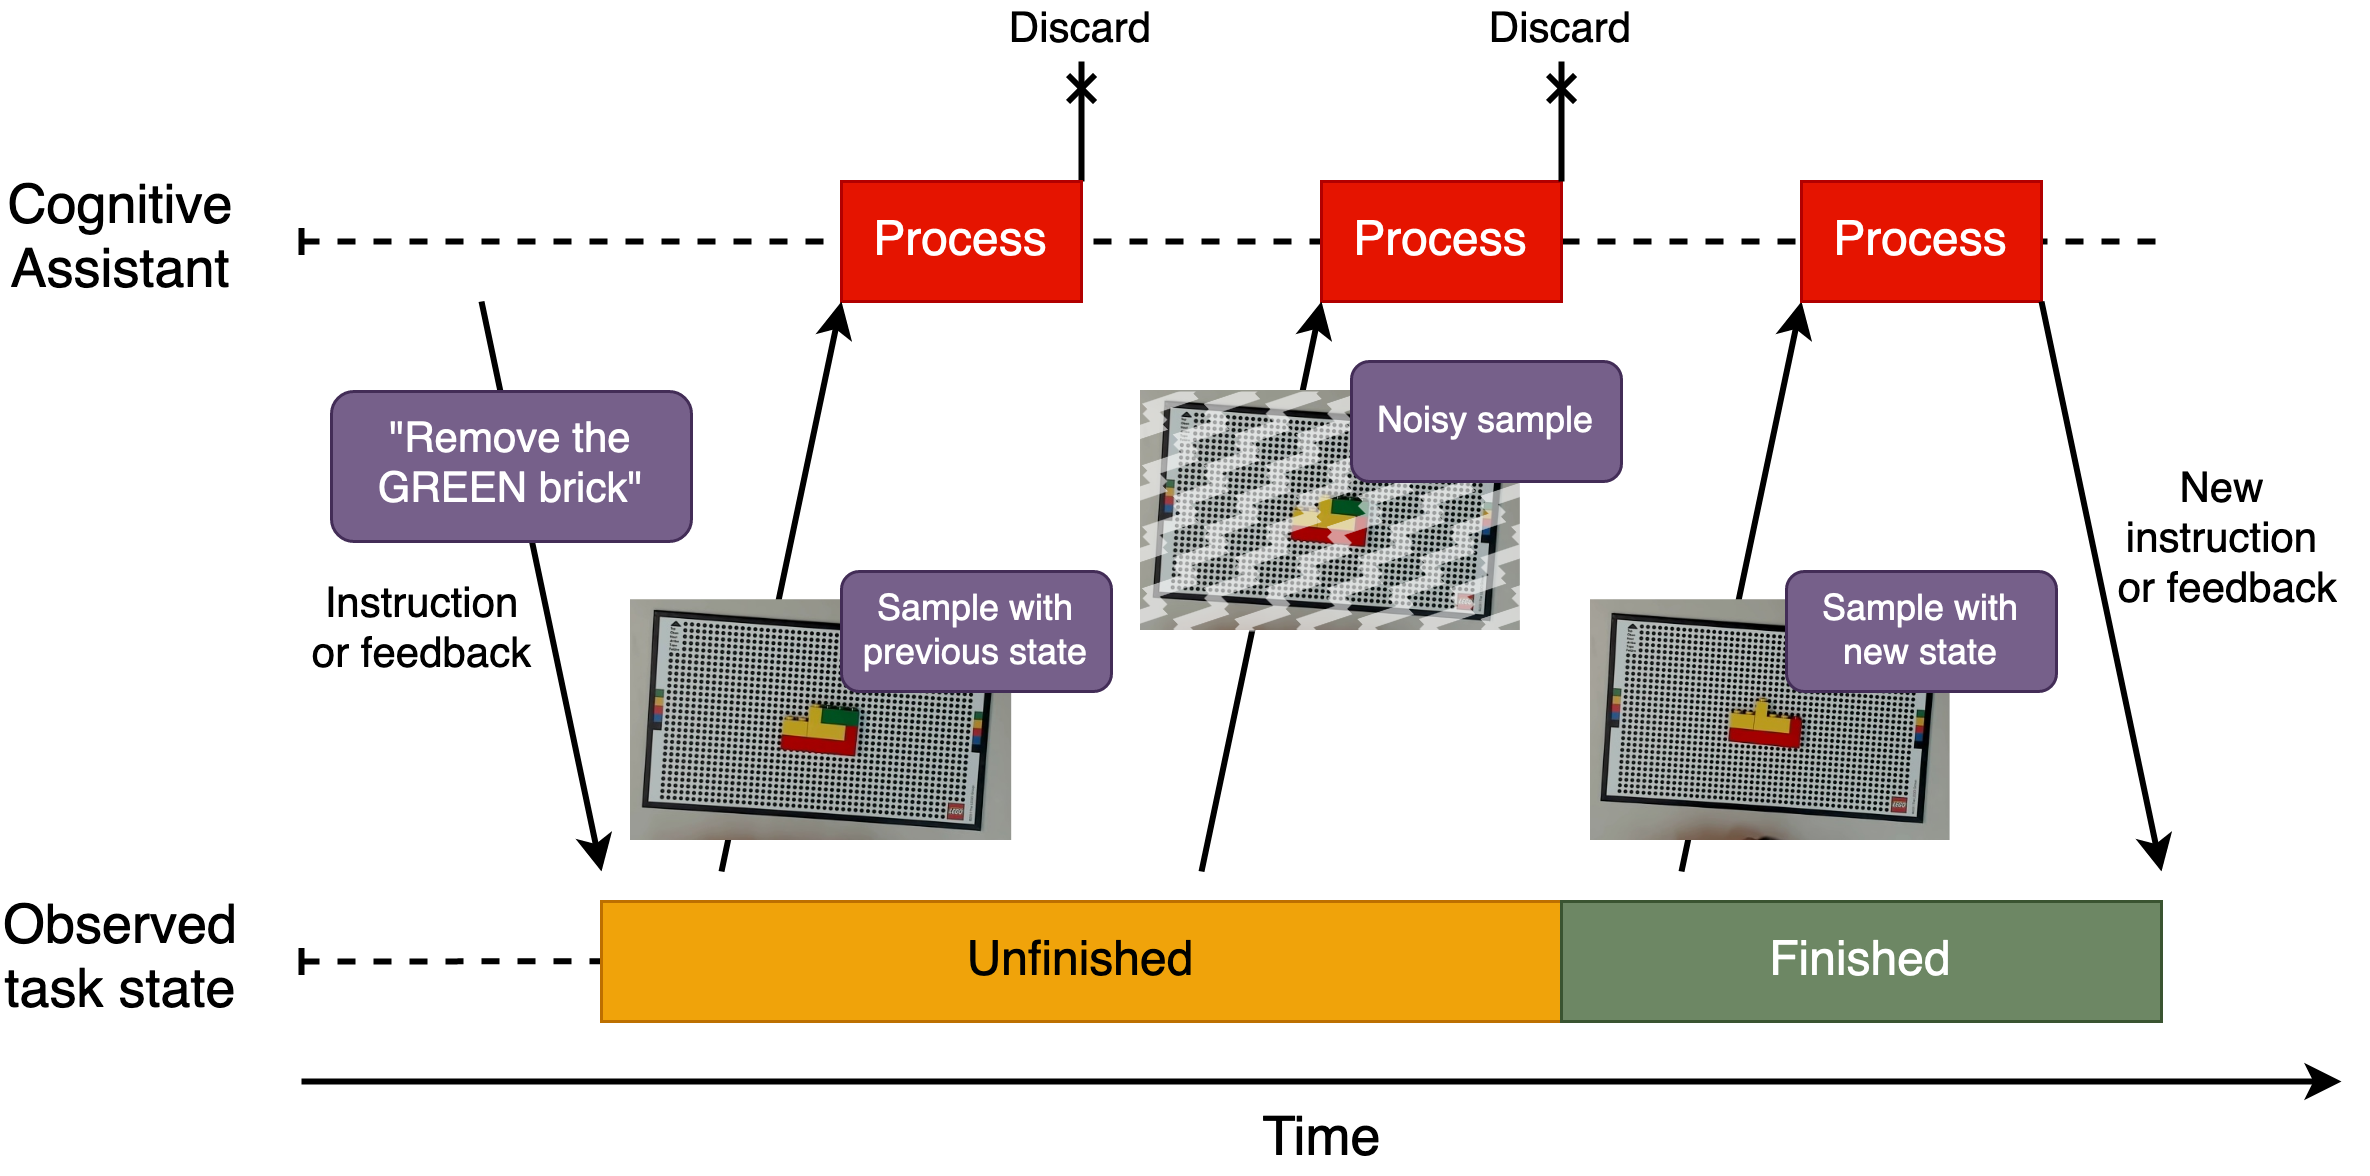
\includegraphics[width=.9\textwidth]{figures/wca_state}
    \caption{Mode of operation of step-based \acs{WCA} applications.}\label{fig:wca:operation}
\end{figure}

In this dissertation, we focus specifically on \emph{step-based} \gls{WCA}.
These applications operate in a manner analogous to how \gls{GPS} navigation assistants guide users, illustrated in \cref{fig:wca:operation}.
The progress of the user is seamlessly and continuously monitored by the application, which provides relevant instructions and feedback only when these are needed.
The application follows the progress of the task in real-time by repeatedly sampling the state of the physical system, most commonly through video feeds.
Whenever the assistant detects a change in the context of the user, it provides a new instruction.
The application otherwise remains silent and out-of-the-way; samples with unfinished states or noise are silently discarded.

This mode of operation has novel consequences for the \gls{QoS} requirements of \gls{WCA} applications.
As with general \gls{AR}, \gls{WCA} has relatively lax bandwidth requirements; however, latency requirements in \gls{WCA} can vary along the execution time of the application.
Users of these applications can only notice system responsiveness when they are \emph{expecting} feedback, that is, immediately after the completion of a logical step or instruction.
Latency bounds can thus be very lax immediately after an instruction is generated (as no feedback is expected yet), and on the other hand much more stringent right after the user has completed an instruction.
In turn, this leads to interesting opportunities for resource consumption optimization in \gls{WCA} applications, such as the adaptive sampling scheme proposed in~\cite{wang2019towards}.
The fact that users \emph{consciously} expect near-instantaneous feedback immediately after finishing an instruction also leads to strong and cumulative reactions to delays in the system, as evidenced by our work in \cref{paper:olguinmunoz2021impact}, implying that careful consideration to latencies must be taken when designing these systems.

\subsubsection{\glsfmtlongpl{CPS}}
\glsreset{CPS}

The term \gls{CPS} applies to a range of systems in which the computational world is tightly integrated with the physical world.
\glspl{CPS} are designed to monitor, control, and optimize physical processes.
By continuously monitoring and analyzing data from the physical components, \gls{CPS} can make decisions and take actions to optimize the system's performance.
For example, a \gls{CPS} controlling a building's heating, ventilation, and air conditioning system may adjust the temperature based on occupancy patterns, external weather conditions, and energy consumption goals.

\glspl{CPS} have acquired increasing importance in a wide range of industries due to their potential to enable greater efficiency, safety, and reliability in complex processes.
Examples of such applications of \glspl{CPS} include smart grids, \acs{ITS} and autonomous vehicles, and smart health monitoring.
A \emph{smart grid} is a \gls{CPS} that enables two-way communication between power generation, distribution, and consumption systems.
Smart grids can thus dynamically and in real-time adjust the distribution of power based on demand and supply conditions.
\glsreset{ITS} An \gls{ITS} is a system that integrates compute, monitoring, and communication in the context of a transportation system.
\glspl{ITS} enable real-time traffic monitoring and management, route optimization, and integration of autonomous vehicles.
These systems aim to optimize the management of transportation infrastructure and improve the safety, efficiency, and reliability of transportation systems.
Finally, \emph{smart health monitoring} is an application of \glspl{CPS} in which wearable devices equipped with sensors and communication capabilities collect real-time data on patients' vital signs, activity levels, and medication adherence.
This data can then be analyzed to provide alerts to healthcare providers, improve diagnoses, and facilitate early intervention.

Although these systems can enable greater efficiency, safety, and reliability in complex processes, the adoption of \glspl{CPS} faces several technical, social, and regulatory issues.
One of the key technical challenges relates to the reliability and safety of \glspl{CPS}.
As these systems tightly integrate physical and computational components, a failure in one component can have significant consequences.
As exemplified above, key use-cases for \glspl{CPS} include critical infrastructure such as power grids, transportation systems, and healthcare monitoring systems.
Any failure in these systems can have serious consequences for public safety and well-being.
Furthermore, \glspl{CPS} require strict security and confidentiality, given the sensitive data in these systems.
Developing CPS that are resilient to attacks and failures, as well as developing methods for testing and verifying their safety, is therefore a major research challenge.

\paragraph{\glsfmtlongpl{NCS}}\label{background:ncs}
\glsreset{NCS}

A research topic within \glspl{CPS} that is of particular interest to this dissertation is \glspl{NCS}. 
A control system is a collection of devices or subsystems that work together to achieve a desired behavior or outcome of a physical system.
These systems are composed of
\begin{inlineenum}
    \item a \emph{plant}
    \item \emph{sensors}
    \item \emph{actuators}
    \item a \emph{controller}
\end{inlineenum}.
Plant refers to the physical system being controlled.
Sensors sample and encode the state of the plant and transmit it to the controller.
The controller processes these inputs, and generates control signals to be sent to the actuators, which modify the plant's behavior.
The overall goal of a control system is to regulate a process or a physical system to meet desired specifications or objectives, such as maintaining a constant temperature, tracking a set trajectory, or regulating the speed of a machine.

\gls{NCS} research is a research direction in the field of automatic control that focuses on the study and development of control systems that formally account for the effects of incorporating communication networks for data exchange between different components of the system.
Every modern control system is, to some extent, networked in the sense that a communication medium is used to transmit information between components.
The field of \gls{NCS} research formalizes and extends this characteristic by integrating traditional control systems with general-purpose \acs{TCP}/\acs{IP} networks.
\glspl{NCS}~\cite{gupta2010networked} aim to enhance and extend the capabilities of traditional control systems by decoupling the controller from the plant, sensors, and actuators (see \cref{fig:csvsncs}).
This allows for remote monitoring and control, which enhances the reliability and safety of the control system
This is particularly useful in applications where real-time monitoring and control are critical, such as in industrial automation and in transportation systems.
\glspl{NCS} also enable the integration of multiple control systems, as well as centralized control of multiple plants by a single controller.
This leads to enhanced scalability and flexibility, and allows improved coordination and collaboration among systems.
Furthermore, \glspl{NCS} provide greater access to information, as they enable the exchange of data and information between control components and systems, leading to more informed decision-making and improved performance.

\begin{figure}
    \centering
    \begin{subfigure}[t]{0.45\textwidth}
        \centering
        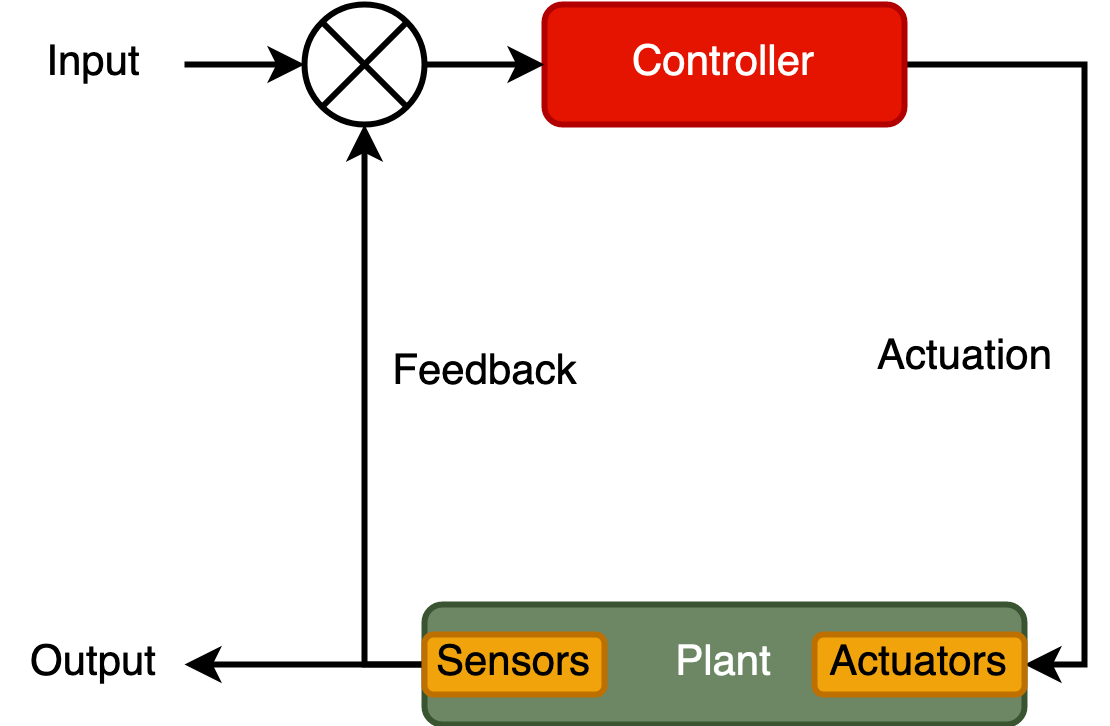
\includegraphics[width=\textwidth]{Figs/control_system}
        \caption{%
            Traditional control system.
        }
    \end{subfigure}%
    \hfill%
    \begin{subfigure}[t]{0.50\textwidth}
        \centering
        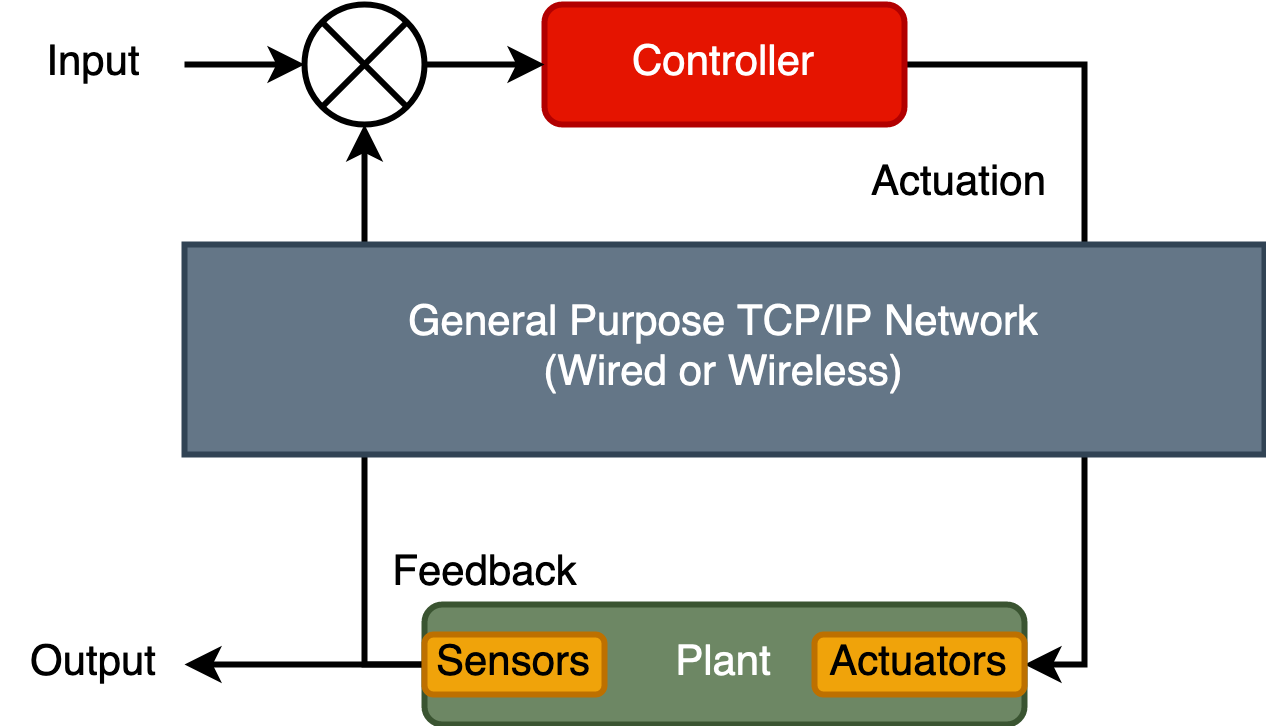
\includegraphics[width=\textwidth]{Figs/networked_control_system}
        \caption{%
            \acl{NCS}.
        }
    \end{subfigure}
    \caption{%
        Comparison between traditional control systems and \aclp{NCS}.
        In an \aclp{NCS}, controller and plant are physically separated and both actuation commands and sensor inputs are shared through a general purpose \acs{TCP}/\acs{IP} network.
    }\label{fig:csvsncs}
\end{figure}

% Please add the following required packages to your document preamble:
% \usepackage{booktabs}
\begin{table}[t]
    \centering
    \caption{Examples of use cases for NCS and their respective latency and reliability requirements.}\label{tab:controlsystemqos}
    \tiny
    \renewcommand{\arraystretch}{1.5}
    \begin{tabularx}{\textwidth}{@{}lYcX@{}}
        \toprule
        \textbf{} & \bfseries\makecell{Sampling~Rate} & \bfseries\makecell{Latency\\Bounds} & \bfseries\makecell{Reliability\\Requirements} \\ \midrule
        \bfseries\makecell[l]{Power\\Electronics} & Up to several \unit{\kilo\hertz} & \textless~\SI{1}{\milli\second} & High; failures can lead to damage to expensive equipment, large-scale blackouts. \\
        \bfseries\makecell[l]{Autonomous\\Vehicles} & Up to hundreds of \unit{\hertz} & \textless~\SI{10}{\milli\second} & High; failures can lead to injury or death. \\
        \bfseries\makecell[l]{Industrial\\Automation} & From sub-\SI{1}{\hertz} to several \unit{\kilo\hertz}. & \SI{1}{\second} to sub-\SI{1}{\milli\second} & High; failures can lead to injuries and/or significant impairment of production and loss of revenue. \\
        \bfseries\makecell[l]{Robotics} & Up to several \unit{\kilo\hertz} & \textless~\SI{1}{\milli\second} & Low to high, depending on the application. \\ \bottomrule
    \end{tabularx}
\end{table}

\glspl{NCS} have become increasingly popular in recent years due to advances in communication and control technologies, as well as the increasing demand for real-time, remote, and distributed control.
They have found use in varied applications, such as industrial automation, transportation systems, and smart buildings, and some have attempted to leverage the Cloud for centralized, distributed control in what has been called \emph{Cloud control systems}~\cite{xia2015cloud}
However, \glspl{NCS} can have timing requirements for communication that conventional Cloud paradigms simply cannot meet~\cite{wan2020efficient}.
Depending on the system being controlled, control systems can have sampling rates ranging from sub-\SI{1}{\hertz} to several \unit{\kilo\hertz}.
Reliability is another concern, as many of the core use cases for \gls{NCS} involve application domains in which failure has the potential to cause bodily harm to humans or significant financial losses.
\cref{tab:controlsystemqos} lists some example use cases for \gls{NCS} and their \gls{QoS} requirements.
These stringent requirements have led their adoption to be limited mostly to industrial environments.
This is about to change, however, as with the advent of \gls{MEC}, consumer-grade \glspl{NCS} will be made possible.
This technology will likely become the backbone of consumer-grade, widely-deployed \glspl{NCS}, enabling real-time capabilities through extremely low end-to-end latencies together with context- and locality-awareness.
